\documentclass[fleqn]{MJDArticle}
%%%%%%%%%%%%%%%%%%%%%%%%%%%%%%%%%%%%%%%%%%%%%%%%%%%%%%%%%%%%%%%%%%%%%%%
\begin{document}
\titleAT[Abstract Outline]{Matthew Denny}

\section{Gender in Organizations}

\begin{enumerate}
	\item Gender bias in organizations is well documented in terms of pay, prestige, position, and social interaction. 
	\item Gender equity is normatively important.
	\item Scholars have sought to understand the roots of gender bias, but have not had access to much behavioral data.
	\item With the increasing use of electronic communication, and the rise of e-government/ transparency, we are now able to use government email to study gender bias using behavioral data.
	\item Therefore, we choose to explore the relationship between gender and communication patterns in government organizations.  
	\item To do this, we collect and analyze large scale email data from a sample of 17 local governments.  
\end{enumerate}

\section{Data}

\begin{enumerate}
	\item North Carolina has robust public records laws which let us collect data.
	\item We did this as part of a transparency-by-conformity field experiment.
	\item 17 counties participated, allowing us to compare across organizations.
	\item Provide some descriptive statistics of the data.
	\begin{figure}[H]
		\centering
	\caption{\label{fig:nc map} North Carolina county map.}	
	\centering
	
\includegraphics[width = 0.48\textwidth]{images/County_Map.pdf}
	\end{figure}
	
	\begin{table}[H]
	\centering
		\begin{tabular}{lrrrrr}
		  \hline
		 \textbf{County} & \textbf{Mgrs.} & \textbf{Female} & \textbf{Internal} &\textbf{Total} \\
		  \hline
		Alexander & 21 & 9 & 907 & 11,924  \\
		Caldwell & 20 & 8 & 121 &    \\
		Chowan & 23 & 11 & 2,027 & 11,737  \\
		Columbus & 24 & 10 & 920 & 12,707  \\
		Dare & 27 & 12 & 2,247 &   \\
		Duplin & 27 & 14 & 1,914 &   \\
		Hoke & 24 & 11 & 1,106 & 5,565  \\
		Jackson & 24 & 6 & 1,499 &   \\
		Lenoir & 20 & 5 & 560 & 10,499 \\
		Lincoln & 22 & 7 & 573 & 8,727  \\
		McDowell & 17 & 5 & 326 & 3,494  \\
		Montgomery & 18 & 10 & 680 & 2,465  \\
		Nash & 19 & 8 & 1,147 & 9,133 \\
		Person & 21 & 9 & 1,491 & 14023  \\
		Transylvania & 20 & 4 & 1,857 & 14,088 \\
		Vance & 18 & 8 & 185 & 4,349  \\
		Wilkes & 17 & 2 & 303 & 8,443  \\
		   \hline
		   \textbf{Totals:} & 362 & 139 & 17,863 & 117,154  \\
		   \hline
		\end{tabular}
		\caption{\label{tab:county aggregate stats}Participating county email statistics. \textbf{Mgrs.} is the total number of department managers in a county, \textbf{Female} is the number of female managers in that county, \textbf{Internal} is the number of emails sent between managers in a county, and \textbf{Total} is the total number of emails sent and received by department managers in each county in our sample. Note that in this study, we only make use of the internal email data. Some email \textbf{Total}'s are omitted due to challenges in determining which emails (not sent by managers) were valid in these counties.}
	\end{table}

	\item These counties are a representative sample and we have tons of data so lets start analyzing it.

\end{enumerate}


\section{Descriptive Analysis}
\begin{enumerate}
	\item If we want to know about gendered patterns of communication in organizations, we should start by looking at aggregate statistics by gender:
	
	
	\begin{table}[H]
	\centering
		\begin{tabular}{m{2in}rrr}
		\toprule
	& \textbf{Male} & \textbf{Female}  \\
		 \midrule
		 Proportion of Sample & 61.6\%& 38.4\% \\
		 Average Emails Sent & 48.3 & 51 \\
		 Average Emails Received & 70.8 & 71.6 \\
		 Average Recipients Per Email Sent & 1.45 & 1.43 \\
		 Recipients of Emails Sent By Female Managers & 62.2\% & 37.8\% \\
		 Recipients of Emails Sent By Male Managers & 60.7\% & 39.3\%  \\
		\bottomrule
		\end{tabular}
		\caption{\label{tab:email agg stats}Manager email statistics by gender.}
	\end{table}
	
	\item The gender split is 60\% men, 40\% women and they both send and receive a comparable number of emails on average, so no volume difference.
	\item Male and female managers also do not communicate with their own gender at a higher rate. 
	\item No gender bias? One place the literature tells us to look for gender bias is in the roles/positions in the organization.
	
	
	\begin{figure}[H]
	\centering
	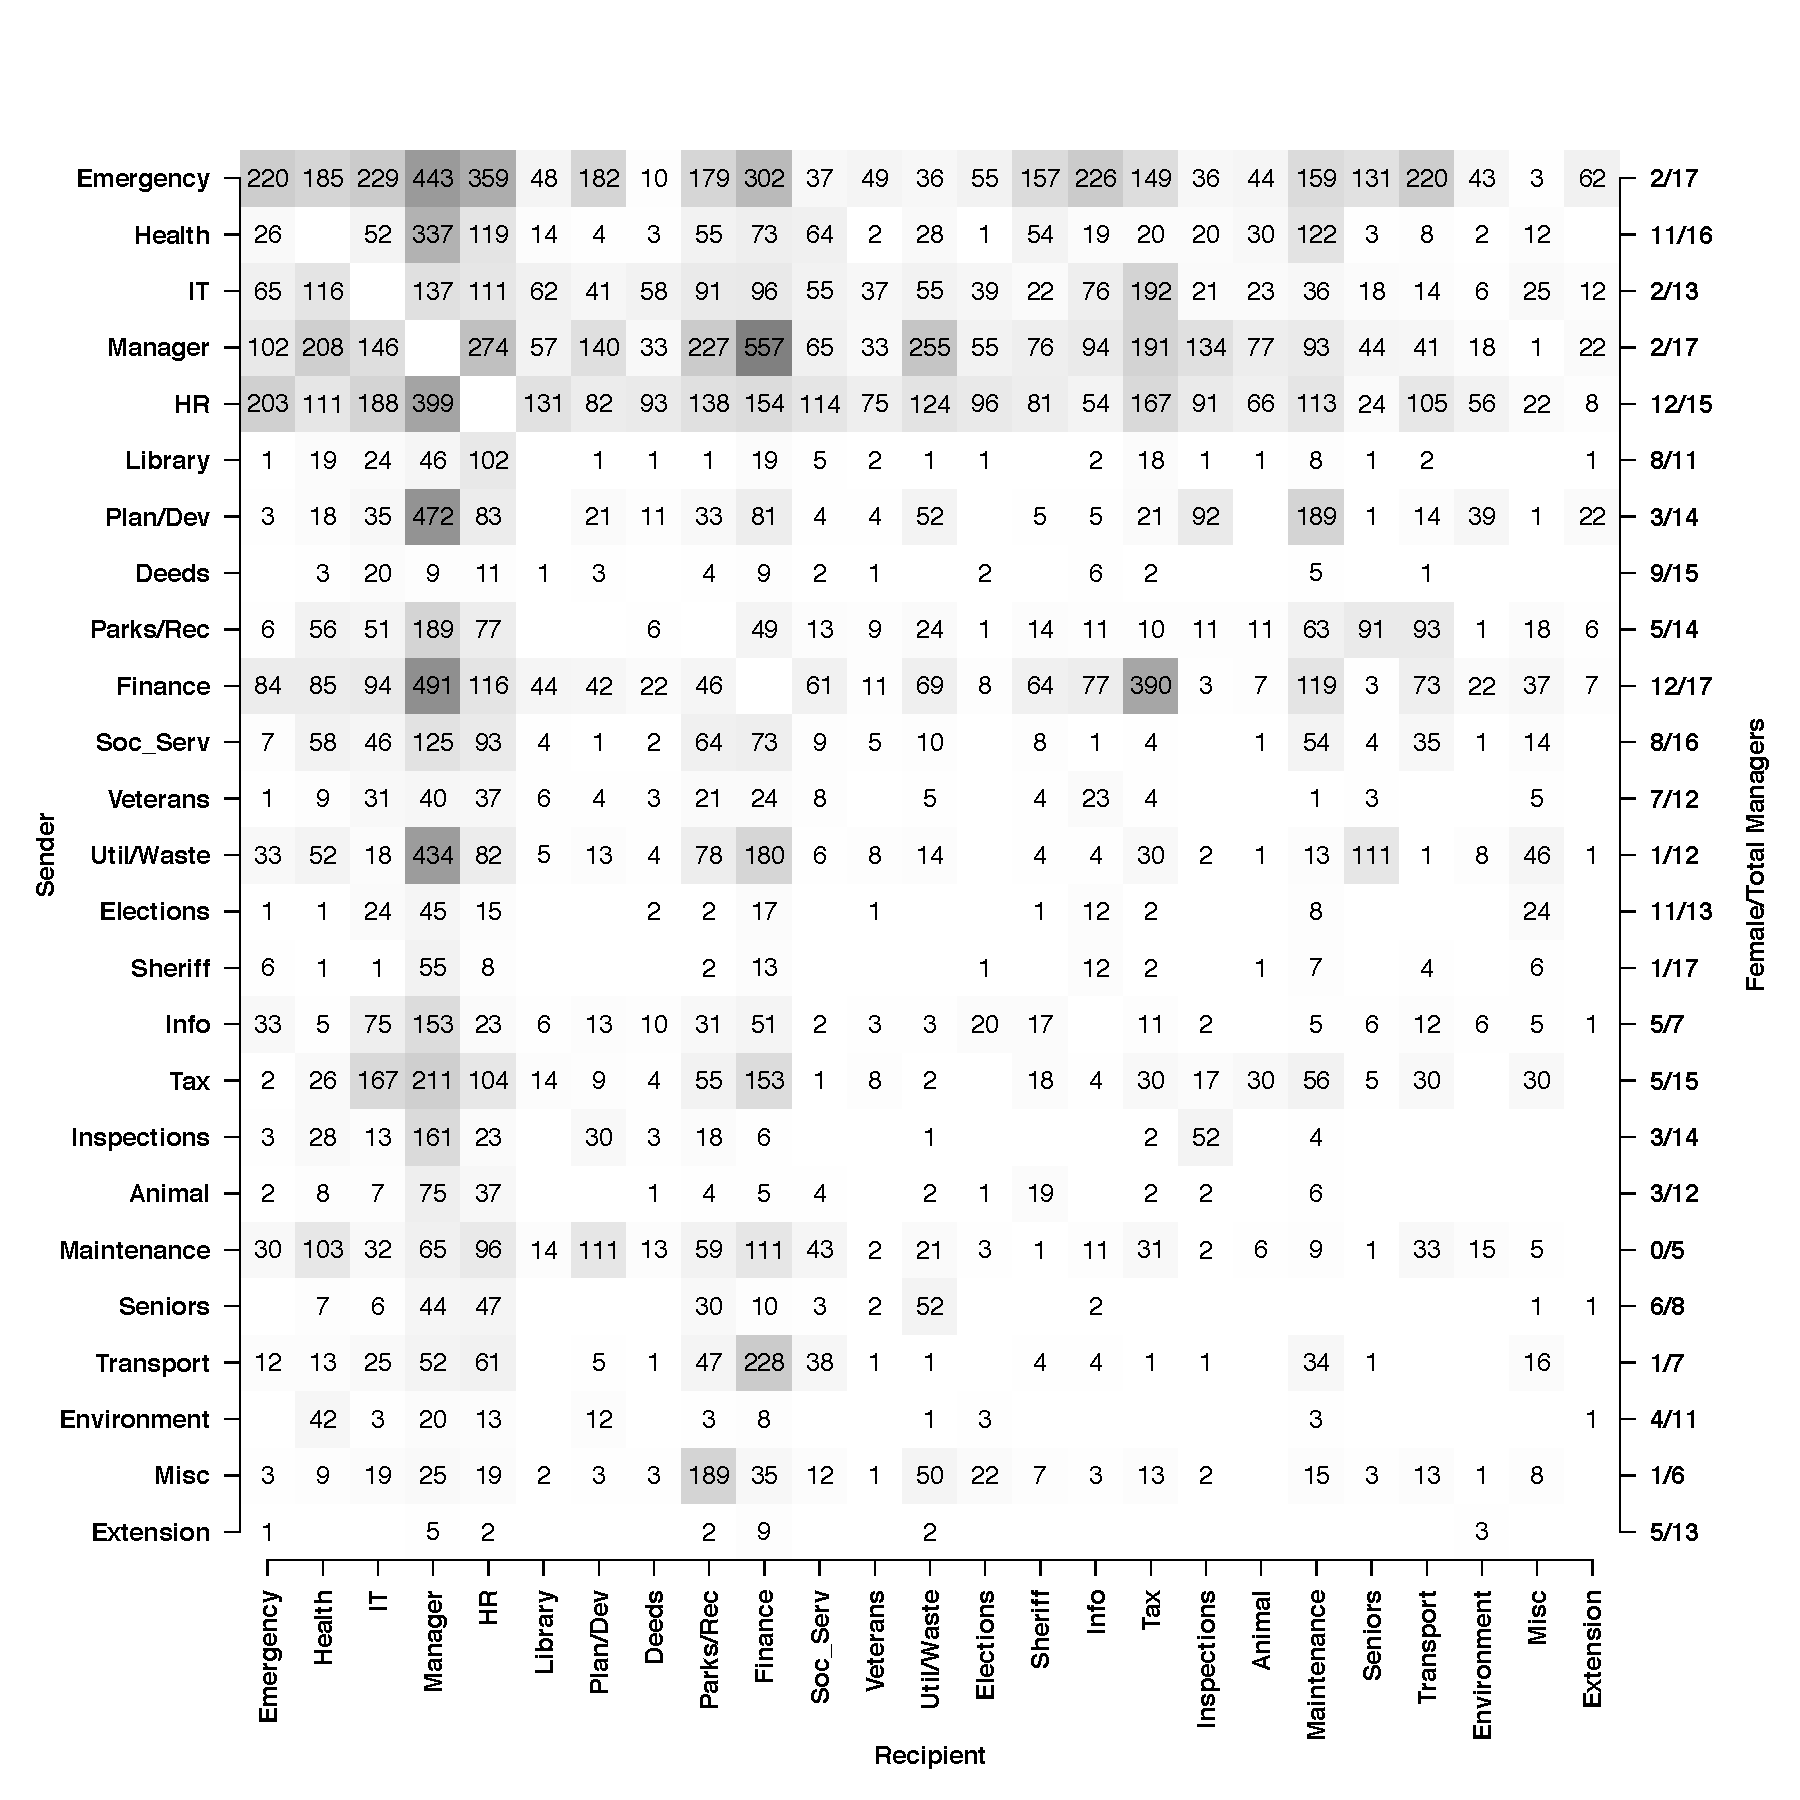
\includegraphics[width = 0.8\textwidth]{images/Aggregate_Email_Flows.pdf}
	\caption{\label{fig:heatmaps}Heat map depicting the number of emails sent from the row department to the column department aggregated across counties. Departments were also hand coded into one of 25 different categories based on given titles, to group departments that perform a similar function. The right margin displays the number of counties that had a manager of type X, and the number of those managers who were women.}
	\end{figure}
	%
	
	\item We can see that some departments are mostly men -- the county manager (the boss), the sheriff, and the emergency manager, for example. Others are mostly women -- the HR, finance, health, for example. 
	
	
	
	
	
	
	\begin{table}[H]
	\centering
	\begin{tabular}{m{2in}rrr}
	\toprule
	 \textbf{Email Content} & \textbf{Male} & \textbf{Female} & \textbf{t-test} \\
	 \midrule
	 Emails Sent to County Manager & 24.4\% & 17.9\% &   \\
	 Average Number of Question Marks Per Email & 0.218 & 0.235 & 0.033\\
	 Average Number of Exclamation Marks Per Email & 0.088 & 0.363 & 0.001\\
	 Average Number of ``Thanks'' Per Email & 0.340 & 0.425 & 0.028 \\
	\bottomrule
	\end{tabular}
		\caption{\label{tab:Gender Aggregate Stats} Manager-to-manager email communication statistics by gender across all departments and all counties. The \textbf{t-test} column reports reports Welch 2-sample t-test $p$ values for difference in means where applicable. When calculating content statistics, only the body text was used so as to avoid double counting subject lines in responses.}
	\end{table}
	
	\begin{enumerate}
		\item Aggregate patterns of communication between genders do not reveal differences by gender. 
	\end{enumerate}
	\item To dig deeper, we examine email sending patterns by department.
	\begin{enumerate}
		\item We see differences in sending and receiving by gender within specific departments. In particular we look at communication between the county manager and department managers by gender.
		\item Male department managers receive a slightly higher proportion  of their emails from the department manager (an overwhelmingly male position) that their female counterparts in the same positions. However, male department managers send a much higher proportion of their emails to the department manager than their female counterparts in the same positions. 
	\end{enumerate}
	\item Set up the need to model topic specific communication patterns with the following question. We do not observe differences in aggregate patterns of communication, but we do observe differences when we look at the department level, why?
	\begin{enumerate}
		\item Either female department managers have a lower preference for communicating with the county manager over email than their male counterparts, or male department managers talk about more/different things with the county manager, explaining the increased volume. 
		\item Since the gender and organizations literature shows that women use formal channels of communication at a higher rate than men \citep{Ragins1989}, the first explanation is unlikely. Thus we are left with a content based explanation.
	\end{enumerate}
\end{enumerate}

\section{A Model of Email Content}
\begin{enumerate}
	\item Motivation for building a model for email data -- who you send an email to depends on what it is about. 
	\item Our solution: a generative model for email topics and recipients. Then discuss the existing TPME model and why we build on it. 
	\item Overview of the generative process in plain english.
	\item Describe the generative process for LDA part of model.
	\item Model based topic clustering.
	\item Explain how draws of message recipients are conditioned on the email topics. 
	\item Describe the generative process for the latent space portion of model.
	\item Summarize the generative process and lead into inference. 
\end{enumerate}

\subsection{Inference}
\begin{enumerate}
	\item We have to invert the generative process to perform inference on the model parameters.
	\item We use block Metropolis Hastings within Gibbs sampling.
	\item A beta R package is available for those interested.
	\item Discuss our model specification and justify our hyper-parameter choices.
\end{enumerate}

\section{Example Model Output}
\begin{enumerate}
	\item Overview of the output produced by our model: topics/top words, topic clusters, LSM parameters. 
	\item Dare county as a particular example -- disaster response to Hurricane Sandy. 
	\item Discuss the example output and the kinds of inferences we might draw about the network structure associated with a particular cluster of topics.
\end{enumerate}

\section{Organization Size, Gender, and Communication}
\begin{enumerate}
	\item Here, we test whether larger organizations exhibit less gender bias, which is something that \cite{Huffman2010} found using longitudinal data from the Employment Opportunity Commission on occupational status and pay. 
	\item The key benefit of using our model in this context: we remove the confounding effect of what is being talked about on the relationship between gender mixing and organization size. For example, it could be that in aggregate, differences in gender mixing across counties are only be related to differences in how those organizations use email. Some might use email for more informal communication (\citep{Ibarra1992} found that informal communication is more homophilous) while others use it for more formal communication, leading to a difference in gender mixing that is unrelated to organization size.
	\item Display plots.
	\item Discuss our results, which indicate that cross-gender communication is most likely in mid-sized organizations. 
\end{enumerate}




\bibliography{PINLab}
\bibliographystyle{chicago}

\end{document}